\chapter{Optimal Control in Two-Dimensional Space}\label{2d}

In this project \footnote{This particular application was completed as part of a group project undertaken by the author along with Evan Lamb and Jason Newton. Parts of this section are re-purposed from the project report.}, the principles of optimal control were applied to the uDrone. In order to simplify the process, the vehicle and world were modeled as a two-dimensional system with one control input. Dynamic programming was used with a cost function that satisfies the mapping goals of the vehicle while minimizing control input. This section lays out the methods, implementation, and results of this particular application.

\section{Methods}
\subsection{Simplification \& Assumptions}
In order to reduce the complexity of this problem, the vehicle and world are modeled in two dimensions. Since the goal of the vehicle is to move in a straight line along the reef in the X-Z plane (where Z is down and X is forward), this is a reasonable assumptions. To further simplify the problem, the forward thrust is assumed to be at a constant value and the only control input is pitch rate. More assumptions were made to simplify the dynamic model, including constant forward drag, no rotational drag, no Coriolis forces, neutral buoyancy, corresponding centers of buoyancy and mass, and discrete state transitions. 

\subsection{Model}
The first step of this project involved generating a model for the uDrone, defining a cost function, and determining constraints. 

% \begin{figure}[t]
%     \centerline{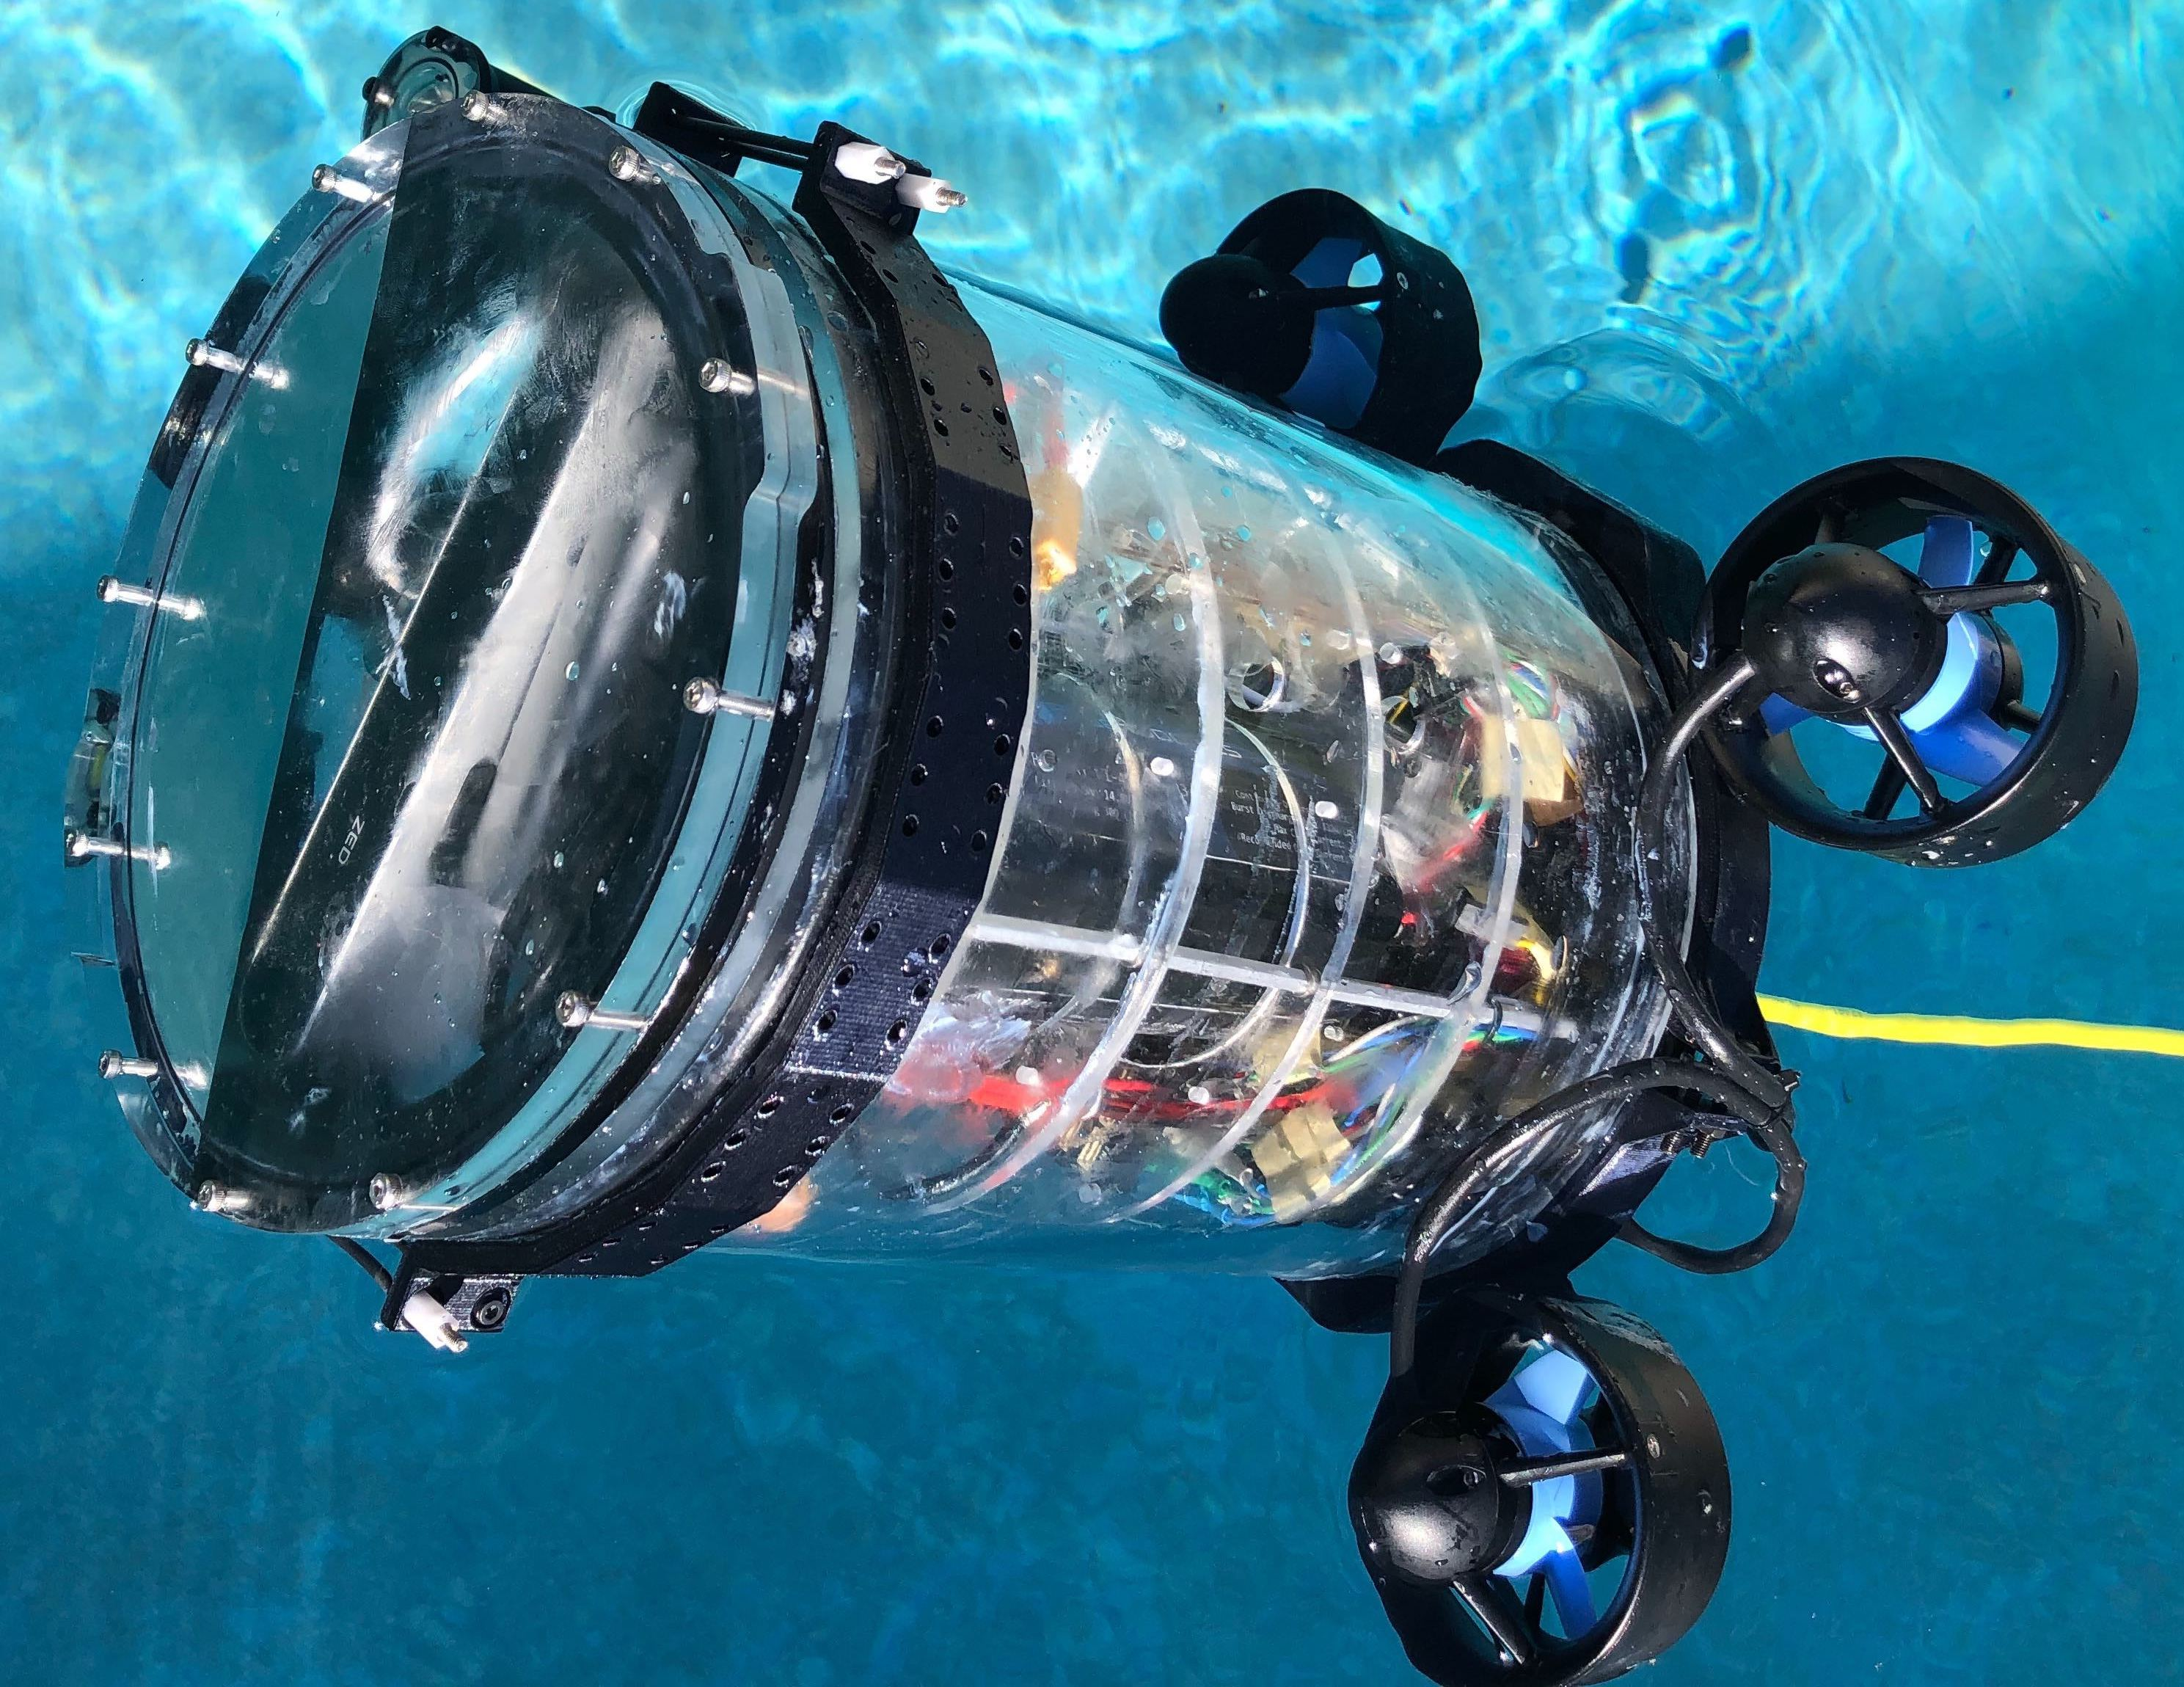
\includegraphics[width=\linewidth]{img/drone_pool.jpg}}
%     \caption{The uDrone}
%     \label{fig:drone}
% \end{figure}
\subsubsection{State Space Equations}
In order to generate state space equations, equations of motion for an underwater vehicle were used \parencite{thor_kin}. 
\begin{equation}
    X=\left[ \begin{matrix} x\\ y\\ \theta \end{matrix} \right], \;\;
    u=\left[ \dot \theta \right]\label{eq:sspace}
\end{equation}
The set of equations \ref{eq:sspace} describe the state space, where $X$ is the state vector and $u$ is the control vector. $x$ is the horizontal position, $y$ is the vertical position, $\theta$ is the pitch, and $\dot \theta$ is the pitch rate of the vehicle. 
\begin{align}
    \begin{split}
        \dot x&=\nu \cos \left( \theta \right) \\
        \dot y&=\nu \sin \left( \theta \right) \\
        \dot \theta&=u
    \end{split} \label{eq:state}
\end{align}
The set of equations \ref{eq:state} are the state space equation where $\dot x, \dot y,$ and $\dot \theta$ are the derivatives of $x, y,$ and $ \theta$ respectively and $v$ is the constant forward velocity.
\begin{align}
    \begin{split}
        x_{k+1}&=v\cos \theta _{k+1}\ast \Delta t+x_{k} \\
        y_{k+1}&=v\sin \theta _{k+1}\ast \Delta t+y_{k} \\
        \theta _{k+1}&= \dot \theta _{k}\ast \Delta t+\theta _{k}
    \end{split}\label{eq:disc}
\end{align}
The set of equations \ref{eq:disc} are the discretized state transition equations to go from time-step $k$ to time-step $k+1$. $\Delta t$ is the length of the time-step. This equation is derived from the state space equations \ref{eq:state}.

\subsubsection{Cost Function}
\begin{align}
    \begin{split}
        J&=\int _{t_{0}}^{t_{f}}\left\| f\left( x\left( \tau \right) \right) -y\left( \tau \right) \right\| ^{2} + \left\| g\left( u\left( \tau \right) \right) \right\| _{R}^{2}d\tau \\
        f\left( x\left( t \right) \right) &\overset{\Delta}{=} \text{desired } y \text{ at given } x\left( t \right)\\
        g\left( u\left( t \right) \right) &\overset{\Delta}{=} \text{motor control cost}\\
    \end{split}\label{eq:cost}
\end{align}
The cost function shown in equation \ref{eq:cost} is a combination of two costs. First, there is the tracking cost which is defined as a vertical deviation from a desired path at any given x value. Its weight is fixed at $Q = 1$. Second, there is the control cost which is defined as the required power output by the uDrone's motors to attain a specific pitch rate. Its weight is varied through three $R$ values: 0.01, 0.05, and 0.1. The function $f \left ( \cdot \right )$ is defined by the desired trajectory. The cost of the motor control is based on the parameters of the motors used in the uDrone \parencite{t200}. The continuous cost function shown above was discretized according to the temporal time step prior to simulation in MATLAB.

\subsubsection{Constraints}
\begin{align}
    \begin{split}
        0\leq & x \leq 10\\
        0\leq & y\leq 4\\
        \frac {-11\pi } {24}\leq & \theta\leq\frac {11\pi } {24}\\
        -70 \leq & \ddot \theta\leq 70
    \end{split}\label{eq:con}
\end{align}
The set of equations \ref{eq:con} show the constraints for the system. The constraints around $x$ and $y$ are based on the problem definition. The constraint on $\theta$ is in place to ensure forward movement of the uDrone and prevent circular references. The constraint on $\ddot \theta$ is based on the motor parameters and model of the uDrone \parencite{t200}. This value is multiplied by $\Delta t$ to determine the constraint on $u$. The constraints were discretized prior to simulation in MATLAB.
\subsection{Dynamic Programming}
To generate an optimal control policy, dynamic programming is used in MATLAB, using the methodology from \parencite{kirk2012optimal}. First, the program initializes all variables and the U*, J* matrices. Using the defined cost function, the cost (J) is computed for each of the final states (i.e. states having $(x=10)$). The code then takes a step backwards in x according to its spatial discretization. The program then computes the "tracking cost" for each state. A higher cost is implemented for going too far beneath the desired path--this is abstracted as hitting the reef. Next, the code checks each of the 15 permissible control inputs at the states and determines 1) what the next state will be based on the state equations, 2) the "control cost" for that control input based on the motor parameters, and 3) the total cost (J) for that choice by adding control cost and tracking cost. Comparing the costs for each of these states, the program chooses the state-action pair with the minimum cost and denotes it as the optimal control. This action is populated into the optimal control (U*) table. The cost associated with this action is populated in the optimal cost (J*) table. This process repeats until it has worked backwards to the initial state $(x=0)$. For each state along $x$, the values for $y, \theta, $ and $u$ are discretized as well.

In a traditional dynamic programming example, the program will use interpolation to determine the J* and U* values at a given state when the state values fall in between the discretized values. Given its high computational cost, interpolation was replaced with a nearest neighbor approach. In this approach, the state being evaluated is simply assigned the J* value of the state which is nearest. Given that we have a 3D grid, this can be likened to landing inside a box with eight corners. These corners represent points at which no interpolation is necessary. Instead of determining the state's exact J*, the program just accepts the J* of the nearest corner and assigns it to the state. 

\section{Implementation \& Simulation}
This section details the specifics of the trials and simulations. Initial trials were conducted at courser discretization resolutions. The trails were made iterative finer until the step size described below was reached.

\subsection{Path}

The path set for the uDrone to follow is based on a piece-wise function shown in equation \ref{eq:pw} and show in figure \ref{fig:path}.

\begin{equation}
y =
    \begin{cases} 
      1 & 0 \leq x < 1 \\
      2-\cos \left( \frac {\pi \left( x-1\right) } {4}\right)  & 1\leq x < 9 \\
      1 & 9 \leq x \leq 10
  \end{cases}\label{eq:pw}
\end{equation}

Additionally, in order to model hitting the reef, any location more than one meter below the curve was given a very high cost.

\begin{figure}[ht]
    \centerline{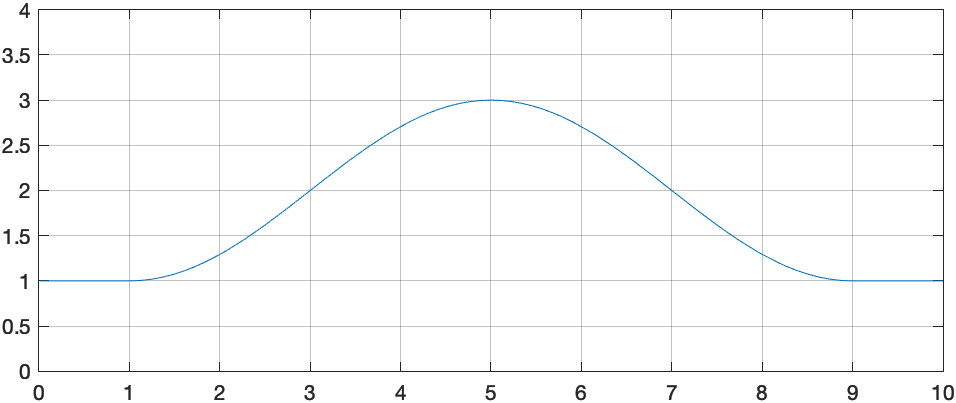
\includegraphics[width=\linewidth]{img/path.png}}
    \caption[Desired uDrone 2D path]{Desired uDrone path in defined state space}
    \label{fig:path}
\end{figure}

\subsection{Cost Function Parameters}

The cost function was determined directly from the motor parameters for the uDrone \parencite{t200}. Specifically, the force needed to pitch the vehicle was used to determine the angular velocity. The power necessary to create this force value is the control cost. Two methods were used for determining the cost, which are called "True" and "Zeroed" in this paper. The true method uses the exact motor values, including the constant force to move the vehicle forward. Therefore, this method takes into account drag. The zeroed approach normalizes the control cost to zero when there is no control input. This method will minimize control action, but not necessarily penalize the vehicle for following a path more closely if it also causes the vehicles to have a lower velocity in the X direction. The control cost curves can be seen in figure \ref{fig:cost}.

\begin{figure}[ht]
    \centerline{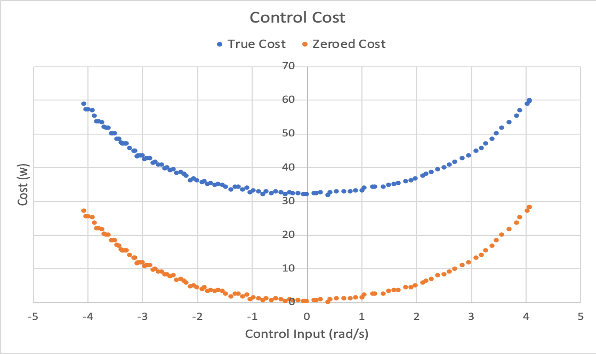
\includegraphics[width=\linewidth]{img/cost.png}}
    \caption[Control Cost]{Control cost for true (blue) and zeroed (orange) methods}
    \label{fig:cost}
\end{figure}

The ratio between control cost and tracking cost weight ($R$) was tested at three values, 0.01, 0.05, and 0.1. Since the values for control cost are in the double digit order of magnitudes and the value for tracking cost are in the single digit order of magnitudes, an $R$ value of 0.1 will treat the two costs as roughly equal. An $R$ value of 0.01 will make the tracking cost 10 times more important than control cost. 

\subsection{Discretization}
When discretizing, first a coarse trial was run at 10 Hz. After this was successful, more fine trials were run, up to 20 Hz. This timestep drove the step size for other variables via the constraint on moving forward in equation \ref{eq:dx}.
\begin{equation}
    \Delta x \leq v \cos \theta _{max} * \Delta t
    \label{eq:dx}
\end{equation}
Additionally, from the timestep the limits on control input are established, as seen in equation \ref{eq:control}.
\begin{equation}
\begin{split}
    \dot \theta = \Delta t * \ddot \theta\\
    -3.5 \leq \dot \theta\leq 3.5
\end{split}\label{eq:control}
\end{equation}
This, along with a desire to maintain fine discretization for grater accuracy, led to the final decision for discrete steps, as shown in table
\begin{center}
 \begin{tabular}{||c c c||} 
 \hline
 Value & Step Size & Step Count \\ [0.5ex] 
 \hline\hline
 x & 0.005 m & 2001 \\ 
 \hline
 y & 0.01 m & 401 \\
 \hline
 $\theta$ & $\frac{\pi}{24}$ rad & 23 \\
 \hline
 U & 0.05 $\frac{rad}{s}$ & 15\\
 \hline
\end{tabular}
\end{center}

\begin{figure}[t]
\centering
\subfigure{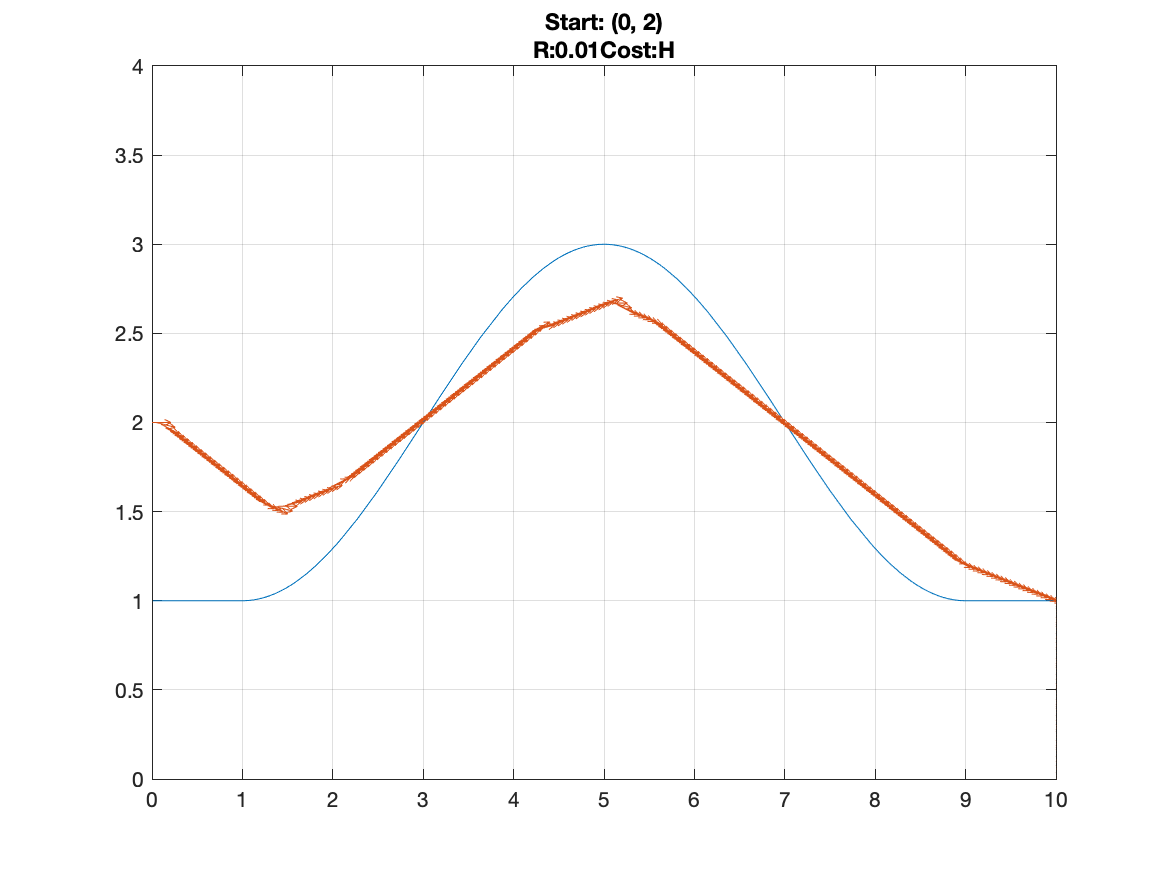
\includegraphics[width=0.32\linewidth]{img/R0_01_true.png}}
\subfigure{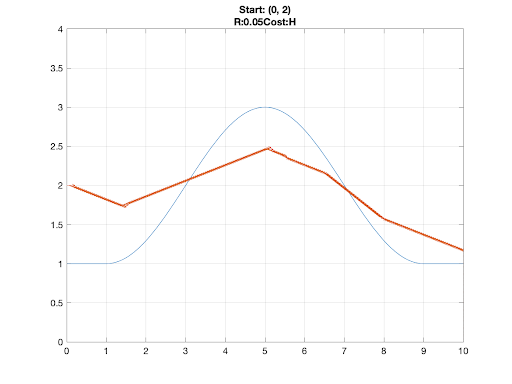
\includegraphics[width=0.32\linewidth]{img/R0_05_true.png}}
\subfigure{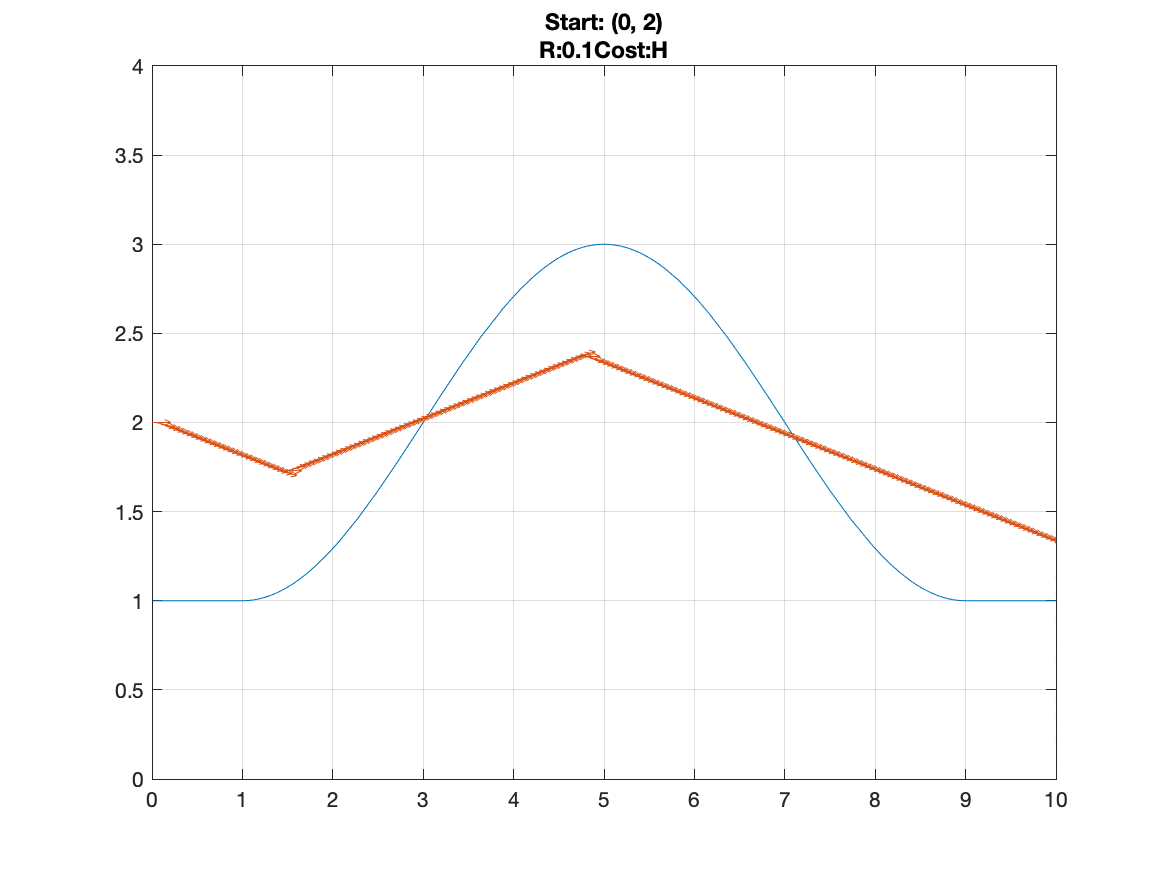
\includegraphics[width=0.32\linewidth]{img/R0_1_true.png}}
\caption[Optimal path using true cost]{Optimal path using true cost method for various R values (Left) R = 0.01 (Center) R = 0.05 (Right) R = 0.1}
\label{fig:true}
\end{figure}

\begin{figure}[t]
\centering
\subfigure{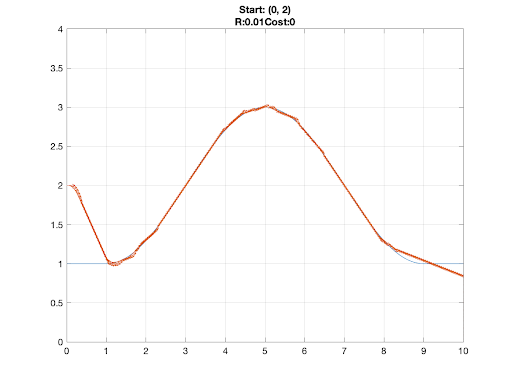
\includegraphics[width=0.32\linewidth]{img/R0_01_zero.png}}
\subfigure{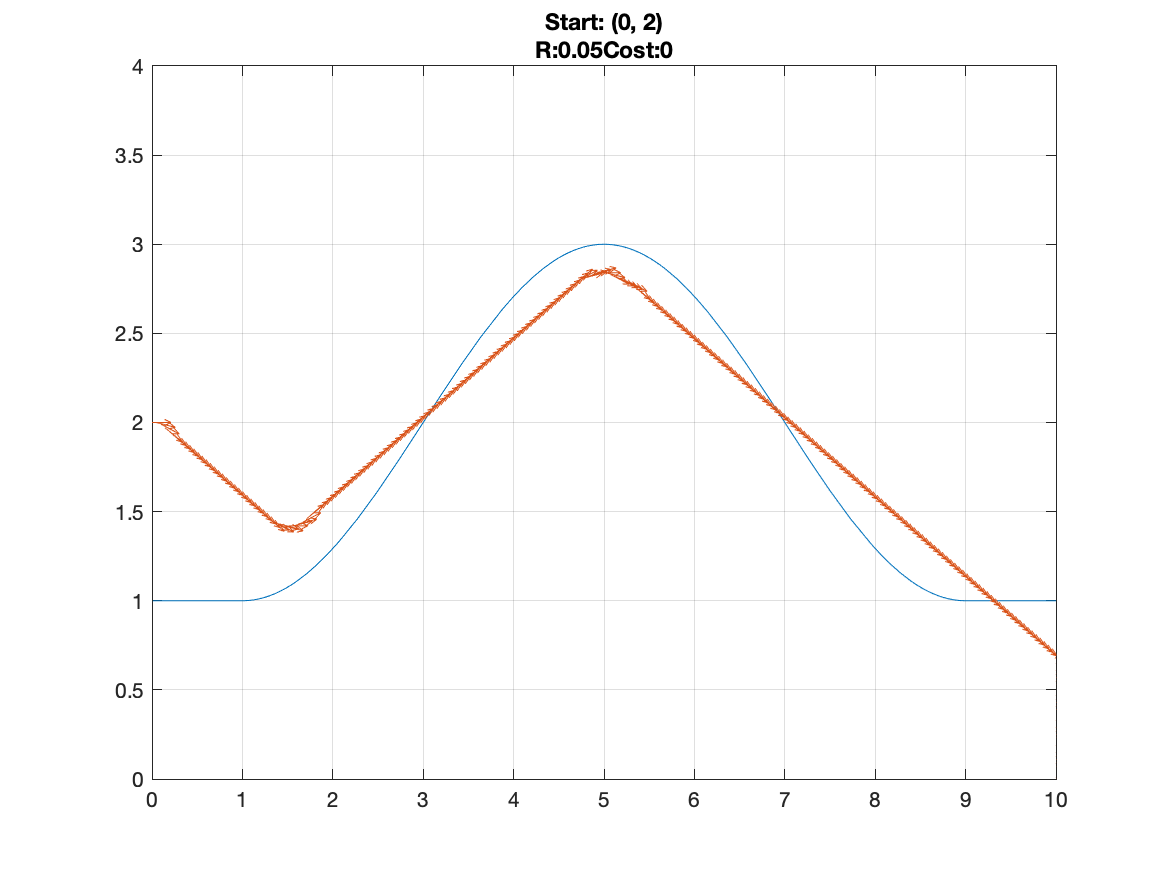
\includegraphics[width=0.32\linewidth]{img/R0_05_zero.png}}
\subfigure{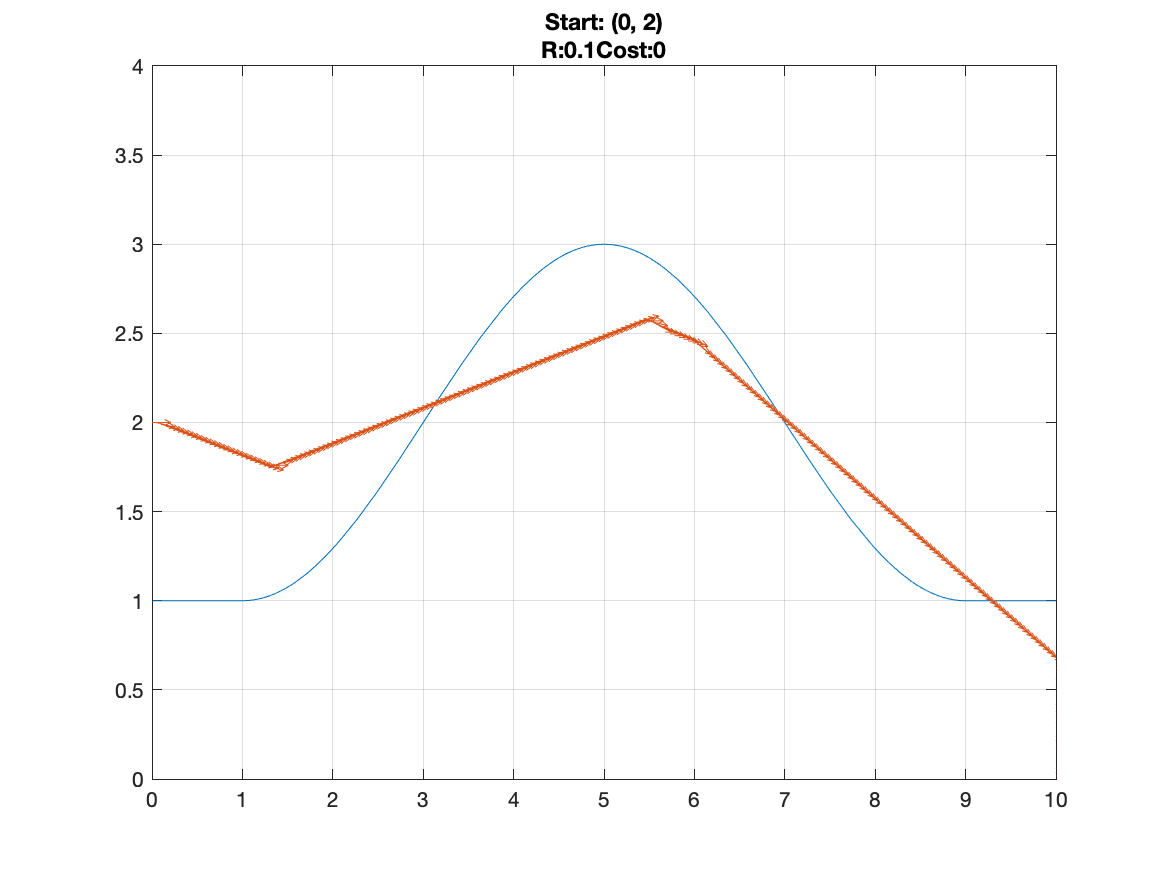
\includegraphics[width=0.32\linewidth]{img/R0_1_zero.png}}
\caption[Optimal path using zero cost]{Optimal path using zero cost method for various R values (Left) R = 0.01 (Center) R = 0.05 (Right) R = 0.1}
\label{fig:zero}
\end{figure}
\section{Results}
Six total trials were run, each with a different cost function method and $R$ value. In each trial 3D optimal cost and optimal control tables are generated. Based on the size of discretization, each table had over 18 million entries and the full trial took approximately 5 hours to complete. Using this data, two graphs are generated: the optimal path and the optimal control law. 
\subsection{Optimal Path}
The first graph demonstrates the optimal path of a vehicle at a given starting point. This is useful for visualizing the vehicle motion and how much it follows the path, as shown in figures \ref{fig:true} and \ref{fig:zero}. There are several conclusions that can be drawn from these figures: 1) As the $R$ value increases, the vehicle deviates from the path more. This can be seen by comparing the graphs in figures \ref{fig:true} and \ref{fig:zero}, where the $R$ value increases from left to right. This makes sense as a lower $R$ value increases the weight of the path following relative to the control cost. 2) The true cost method causes the vehicle to deviate from the path more than the zeroed method. The true cost method also maintains the vehicle at a more horizontal orientation, thus increasing the component velocity in the X direction. This is shown by comparing figure \ref{fig:true} to figure \ref{fig:zero}. The result of the cost method comparison is intuitive since the cost to move forward will cause the optimal path to take the vehicle through the simulation in the least number of steps.

\subsection{Control Law}
The second graph is a visualization of the control law computed by the run. A control law is a table containing the optimal control choice at each state. This table would be loaded on to a vehicle and used to determine control, as running any dynamic programming problem in real time would be to computationally intensive and slow. Since it is not practical to display the full three-dimensional graph in this format, a slice is presented here. Figure \ref{fig:Ustar} shows a single slice of the control law. Specifically, this figure shows the control law for a given $x$ and $y$ when $\theta$ is equal to zero. In this figure the red color represents areas of positive (counterclockwise) optimal control, the blue color areas of negative (clockwise) optimal control, and the white areas of zero optimal control. 

\begin{figure}[h]
    \centerline{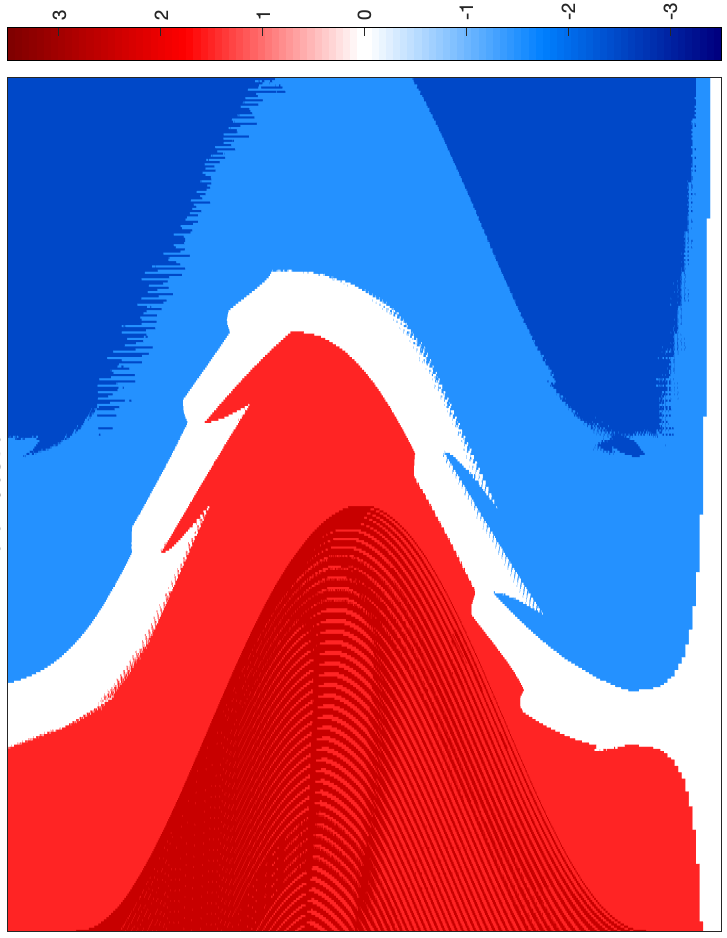
\includegraphics[width=0.5\linewidth]{img/U_star.png}}
    \caption{Optimal Control Law}
    \label{fig:Ustar}
\end{figure}

Clearly visible in the figure is the dark red lower parabola which is the very high cost area of hitting the reef that the control law tries to avoid. The lighter red areas are where the vehicle is behind or below the path and needs to pitch up to get on track. The light and dark blue areas are where the vehicle is above or in front of the path and needs to pitch down. The white band is when the vehicle is directly next to the path and should move straight in the body fixed axes.

% Two main methods of analysis were used - one with zeroed costs and one with the true cost. The true cost accounts for the cost associated with the constant movement of the drone. Since the the drone is always moving at a constant forward speed the true cost method penalized every movement step, so the optimal policy was in part searching for the shortest path. Zeroed cost was also helpful since the only considered input was the pitch rate, so it may be reasonable to ignore the cost of basic forward movements. Both were analyzed for varying values of R. There resulting optimal paths are shown in figure \ref{fig:zero} and in figure \ref{fig:true}. As can be seen, the analysis done with true cost cuts through the set path because there is a cost associated with travel distance. It is therefore optimal to make the trip in the shortest distance possible.




% In addition to plotting the optimal paths a plot showing the optimal control law is shown for each position $X$ and $Y$. where $theta$ is equal to $0$. The map is show in figure \ref{fig:Ustar}. The blue are represents a negative input while red represents a positive input. Note that this specific map is for the case with R = 0.01 and zeroed cost.






\section{Conclusions}
%The key conclusion is that a zeroed cost permits greater path following capacity. This is expected because there is no cost for a control input of 0. In other words, motion is not penalized as heavily in the zeroed cost case as in the true cost case. It is clear in the true cost case that the uDrone simply attempts to exit the grid as quickly as possible without hitting the reef even when $R$ is lowered. When considering the various $R$ values, the results are also as expected. The lower the R value, the greater the permissible control input which manifests itself in the results as greater path following. This is true in the zeroed and true cost cases, but is more evident in the latter case.

This project showed that dynamic programming is a valid method for creating an optimal control law for an underwater vehicle. Since this vehicle's mission is to travel in a straight plane, the simplifications from three to two dimensions would still allow for a usable control law. Additionally, the project showed the effects of the cost function on the optimal control policy. By varying the control cost calculation method (true versus zeroed) and changing the control weights (path following vs. control cost) the optimal trajectory changes. These trade offs need to be weighted based on the specific needs of the vehicle's mission. For example, if mapping fidelity and accuracy is paramount, a low $R$ value and zeroed cost would be best. But, if coverage is more important, a higher $R$ value and the true cost method are best. 

The largest barrier to practical implementation is the compute time and static environment needed for dynamic programming. The compute time issue can be overcome by pre-computing a control law, such as mentioned above. Dynamic programming is useful when the path is known in advance. This occurs when there are existing maps of survey regions or the vehicle is returning to a site it previously visited. However, given the variable topography of reefs, it would be hard to pre-compute a control policy for exploration. In these cases, other optimal methods could be used such as model predictive control or optimal path generation with PID control. 

% Some general conclusions which can be gleaned from these results are: the "nearest neighbor" apprproach sacrifices accuracy in favor of speed, discretization of the states and controls limit smooth action, simple models can yield great intuition, and that zeroing the cost permits greater path following capacity.

% Looking forward to future research, the team would explore this program running onboard the uDrone with a finite horizon. It would require precomputing the J* and U* tables. Other solution methods would also be explored, especially Model Predicitve Control (MPC) and Calculus of Variations.
% \begin{figure}[t]
%     \centerline{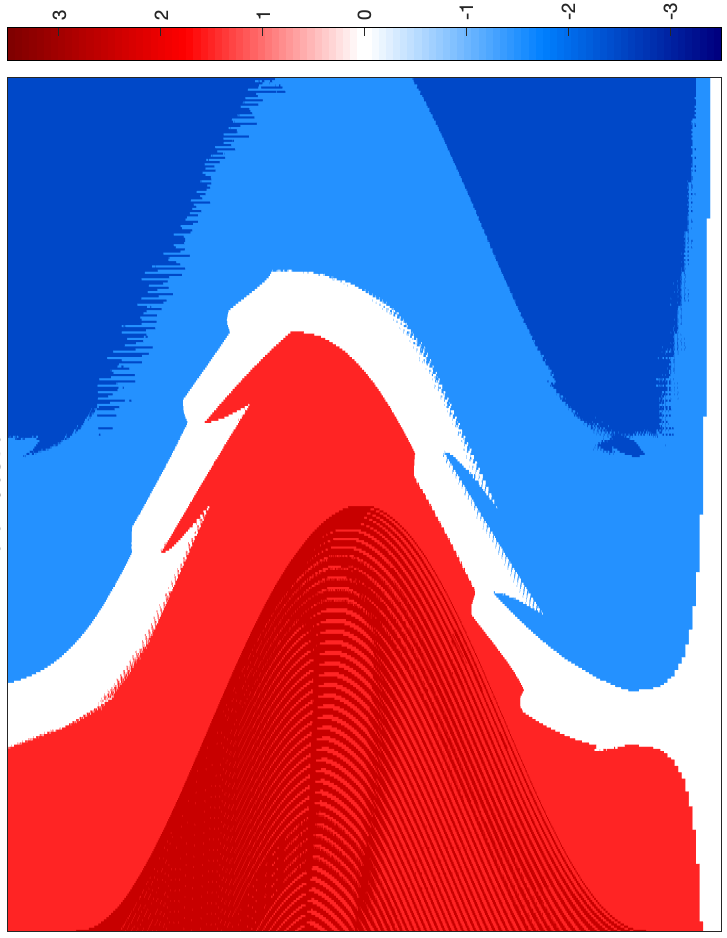
\includegraphics[width=\linewidth]{img/U_star.png}}
%     \caption{Optimal Control Law}
%     \label{fig:Ustar}
% \end{figure}